\documentclass[conference,12pt]{IEEEtran}
\usepackage{pdflscape}
\usepackage{hyperref}
\usepackage{tabularx}
\usepackage{graphicx, subfigure, amsmath} 
\usepackage[backend=biber,style=ieee]{biblatex}
\usepackage[section]{placeins}
\addbibresource{References/References.bib}
\interdisplaylinepenalty=2500

% correct bad hyphenation here
\hyphenation{}


\begin{document}
%
% paper title
\title{RoboTractor}
\author{
\IEEEauthorblockN{Jeremy Wright}
\IEEEauthorblockA{Arizona State University\\jlwrigh1@asu.edu}
\and
\IEEEauthorblockN{Arun Balaji Buduru}
\IEEEauthorblockA{Arizona State University\\abuduru@asu.edu}
\and
\IEEEauthorblockN{David Lucero}
\IEEEauthorblockA{Arizona State University\\dwlucero@asu.edu}
}
\maketitle


\begin{abstract}
The need for the automation of vehicles is increasing due to improved
efficiency and reduced operational costs. Even though the law requires human
presence in self-driven agricultural vehicles, recent trends show that as
our confidence in these self-driven vehicles grow, these requirements on
human presence will be waived. Once we remove humans from control of these
vehicles, secure signaling and control takes center stage as there will be
no human to troubleshoot if the signal and control systems are compromised,
making vehicles vulnerable to be stolen, damaged, or otherwise harmed. The
scope of this project is to build a secure signaling and control system with
mechanisms to drastically reduce if not eliminate these attack vectors. The
main tasks in this project are to build a front-end interface for users to
give instructions built upon a Representational State Transfer (REST)
architecture, set up Extensible Messaging and Presence Protocol (XMPP)
server and client with required authentication and data integrity check
mechanisms, and build a simulated automated vehicle, capable of
interfacing with the XMPP components and front-end.  
\end{abstract}

\begin{IEEEkeywords}
    Secure signaling and control, remote management, agricultural vehicles automation, self-driven vehicles
\end{IEEEkeywords}

\section{Introduction}
Our goal in this project is to build a secure signaling and control system to
enable the effective management of the agricultural vehicles. The primary
problem to be addressed in this project is to securely interface and/or
communicate between user and agricultural vehicles using XMPP and REST
protocols. This is very important because authentication of vehicles and data
integrity, here the path plan and location feedback transmission needs to be
secured and protected from eavesdroppers. This will prevent attackers from
compromising and/or stealing these vehicles. In this project we use Django to
handle the front end interface for the users. We use python libraries to
interface between user and path generator server where we use XMPP and REST
protocols, and XMPP clients to control the agricultural vehicles. We expect to
have a comprehensive tool that translates the abstract user inputs into
executable actions for agricultural vehicles in a secure manner.
\section{System Models}

\subsection{System Model}
RoboTractor will leverage the Django Web framework \autocite{_django_2014}
, to realize the required
interfaces.  Figure~\ref{fig:softwarecomponents} describes the connection of
these components.  The combination of XMPP and REST in RoboTractor is
a demonstration of how to extend the existing HTTP development environment
i.e. "the web of things" into a stateful protocol. HTTP is by design
stateless. XMPP on the other hand is a stateful streaming connection between two
clients. In this case the Tractor and a command server.  To achieve this mesh we
will leverage the Bidirectional-streams Over Synchronous HTTP standard
protocol \autocite{paterson_bidirectional-streams_2010}. BOSH provides
a standard mechanism to operate the streaming XMPP protocol efficiently over an
HTTP connection. This is essential for a scalable webservice. 
\subsection{Software}
\subsubsection{XMPP Server}
RoboTractor uses the ejabberd \autocite{_ejabberd} XMPP server as it provides an existing Python
interface, to integrate with the rest of our Python based ecosystem.
\subsubsection{REST Interface}
TastyPie provides REST \autocite{_toastdriven/django-tastypie_2014} by extending
the existing Django Models.
\subsubsection{BOSH Interchange}
Punjab is an Django plugin implementation of BOSH
\autocite{_twonds/punjab_2014}.  In addition to BOSH, this library combines
the ejabberd Users with Django Users to provide a single authentication and
authorization framework. While this demo project will have a single user type,
this combination is critical to maintain proper use management and
least-privilege authorization.

\begin{figure}
\centering
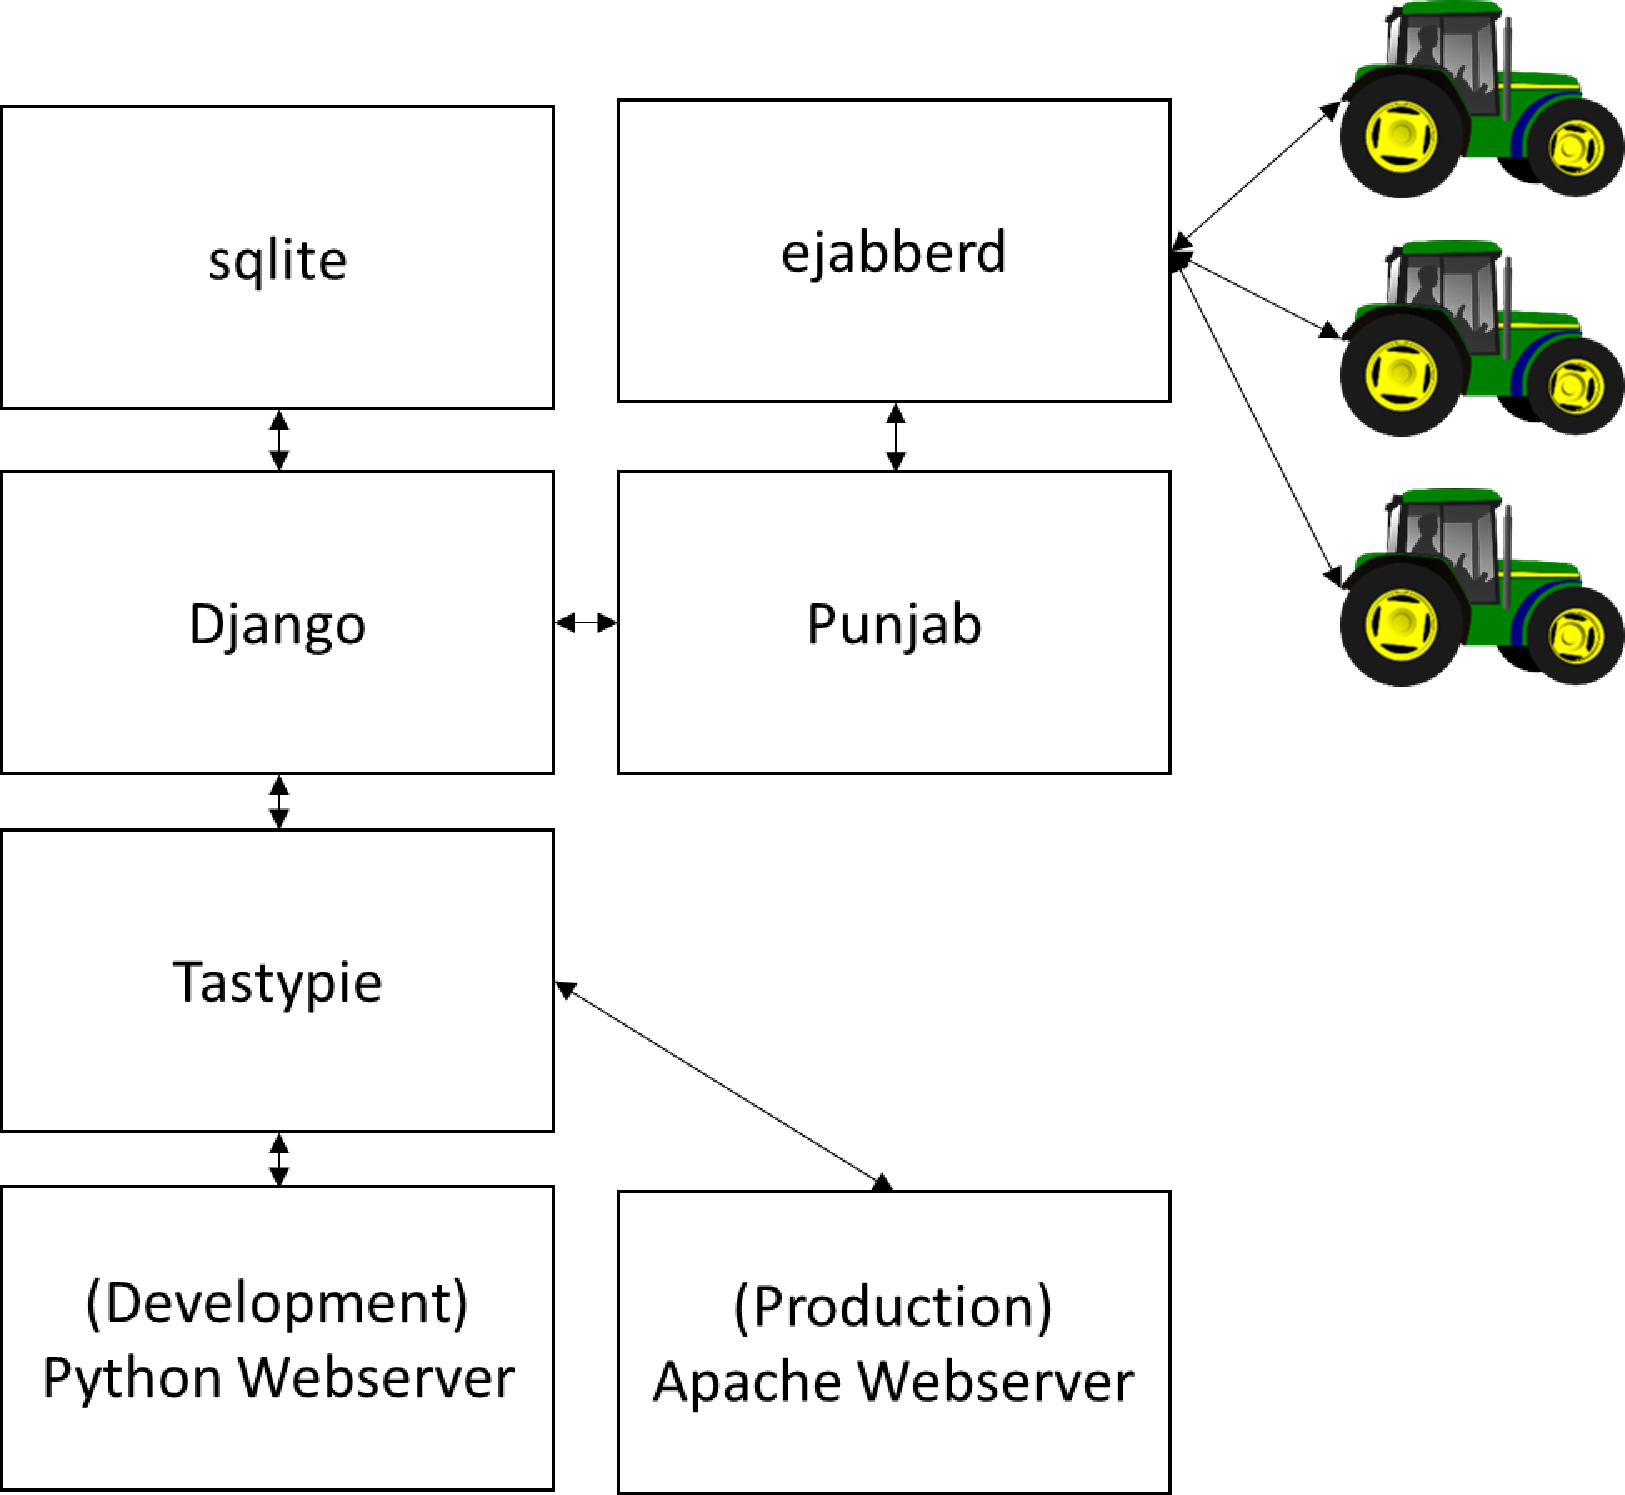
\includegraphics[width=0.4\textwidth]{SoftwareComponentBlockDiagram.pdf}
\caption{Software Component Block Diagram}
\label{fig:softwarecomponents}
\end{figure}

\section{Project Description}
Implementation is divided into 2 primary phases (Marked as milestones on the
attached gantt chart).  The first phase is an integration phase connecting
the various libraries and off the shelf components. It is critical that this
integration does not weaken, but rather strengthens the security properties
provided by each independent component. 

The second phase is the extension of these components to provide command and
control of agricultural vehicles. For schedule mitigation, David and Arun are
scheduled to begin this phase before the framework is assembled. Once the
framework is in place, David and Arun's interface designs may be merged with the
overall system. 
\subsection{Task 1 : Development Environment}
The development environment consists of configuring all the tools needed to
portably work with the software package. This will involve installing project
dependencies, and deployment scripts to allow all members of the team to work
effectively together. The complete environment will be stored in git.
\subsection{Task 2: XMPP Implementation}
XMPP Implementation is a configuration task to setup the ejabberd
server and connect it into the HTTP Framework. Once this is in place the XMPP
Clients may start working.
\subsection{Task 3: Demo Tractor}
The Demo tractor is the complementary component to the Frontend UI. This is the
virtual machine, a piece of software which simulates a real tractor, or
agricultural vehicle. 
\subsection{Task 4: Frontend UI}
The "single-page" web application is the modern design methodology to web apps
today. Leveraging this design architecture the Frontend will query the REST API
to draw the position of all tractors within a Google Map context. This task has
2 high level sub tasks:
\begin{enumerate}
\item Path generation
\item Map rendering
\end{enumerate}
Path generation is the primary deliverable of this project. The user shall be
able to input a path for a given tractor to drive. The Tractor will then receive
this path over the REST to XMPP gateway.  The UI may then periodically query the
position of the tractor and update it on the Google Map.
\subsection{Task 5: Server Backend}
The Server Backend is the critical component which plumbs all the components
together. Extensive knowledge of Django will make this task easier. As it will
require linking multiple components together in a orchestrated fashion.
\subsection{Task 6: REST Interface}
The REST interface will server the primary means of interacting with the site.
The Web interface will exist as a "single-page" app who leverages AJAX
principles over this REST API. 
\subsection{Project Task Allocation}

\begin{figure}
\centering
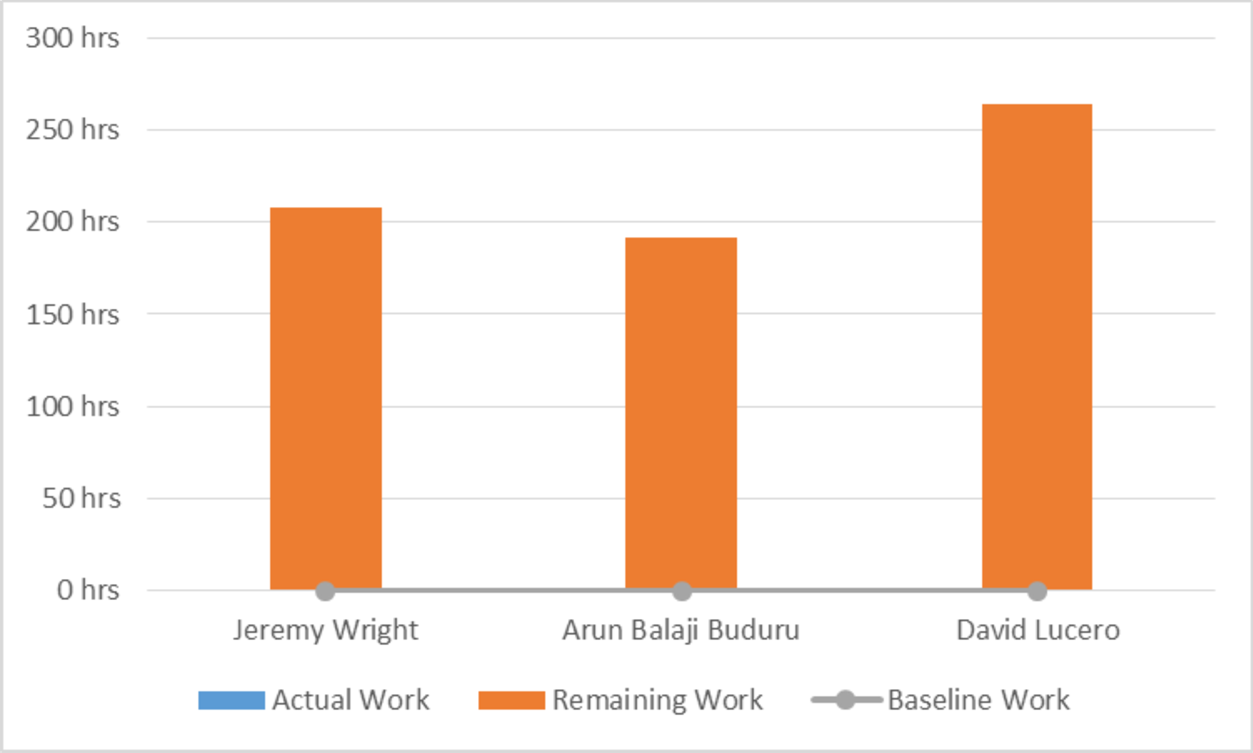
\includegraphics[width=0.4\textwidth]{ResourceAllocation.pdf}
\caption{Resource Allocation}
\label{fig:resourceallocation}
\end{figure}
Jeremy Wright will serve as the project lead since he has past experience with
Python based web applications. 

\subsection{Deliverables}
\begin{enumerate}
\item Web application for sending control commands to remote machine, and
displaying their current location
\item A Simulated vehicle capable of acting on XMPP command send via the Web
interface.
\item An administration panel for configuring vehicles.
\item API documentation for using the REST interface as an external service.
\item API documentation for using the XMPP interface to act as a vehicle.
\end{enumerate}
\subsection{Project Timeline}
The attached project timeline (generated from Microsoft Project) describes the
overall tasks of the project.
\section{Risk Management of the project}
Several potential issues have been identified that may pose risk to successful
completion of this project. These risks have been identified in Table
\ref{tab:riskmanagement}. Along with the description, ratings have been assigned
to each risk identified, and potential mitigation strategies are described.

\section{Conclusion}
In this proposal we intend to build a remote control system leveraging existing
internet technologies XMPP and REST. Future work based on this approach may
include asset management for corporate farm management.

\section{Acknowledgment}
We would like to acknowledge the ASU VLAB for their support of tools and
services for demonstration and development of this project.

\printbibliography
\clearpage
\begin{landscape}
\begin{table}%[!t]
%\renewcommand{\arraystretch}{1.3}
\caption{Risk Management}
\label{tab:riskmanagement}
\centering
\begin{tabular}{c||c||p{2in}||p{2in}}
\hline
\bfseries Risk Description & \bfseries Risk of Failure & \bfseries Consequence of Failure & \bfseries Mitigation Strategy\\
\hline\hline
Connections between components must be secure
& Low
& Product would still function, but would lack security – information assurance will suffer
& Plan to include security on component connections ahead of time. Follow best practices (SSL/TLS)\\
\hline
Evaluation of Project depends on proper vehicle agents
& Medium
& System is unable to be tested if vehicle agents are inoperable or incorrect
& Vehicle agents will be designed first to ensure compatibility with all other components. Thorough review and testing of component to ensure proper functionality\\
\hline
Improper configuration of components
& Medium
& Components do not communicate properly with each other. System functionality is void
& Thorough reviews and testing of components to ensure proper functionality and communication\\
\hline
Incorrect PKI implementation and/or configuration
& Medium
& Puts all identified security domains at risk. PKI used becomes useless. System becomes vulnerable to outside attacks i.e. MITM
& Follow best practices and standards. No re-invention of the wheel\\
\hline
Service Uptime (web reliably)
& High
& Product is unusable if network connections are not operable
& Redundancy. Cloud hosting to alleviate hardware reliance\\
\hline
\end{tabular}
\end{table}
\end{landscape}
\end{document}


